\subsection{Général}
	\begin{itemize}
		\item{Langage utilisé}
		\item{Tout en anglais}
		\item{Modèle Vue Contrôleur}
		\item{Documentation - (Javadoc / appledoc)}
	\end{itemize}
			
\subsection{Menus}

	Au démarrage de l'application vous arrivez sur un menu d'accueil. Depuis
	celui-ci vous pourrez accéder à l'aide, à la liste des comptes locaux ou à la
	création d'un nouveau.
	Les menus de l'application ont été réalisé pour que l'utilisateur ait
	une utilisation intuitive de l'application. Ils se divisent en 4 grandes sections.
		
	Vous avez tout d'abord la section de création de parties locales. Vous aurez
	accès à une liste de cartes ainsi qu'au réglage de difficulté des bots, leur
	nombre et le temps de jeu. Le type de partie sera une fonctionnalité à venir.
	Vous n'aurez plus qu'à créer la partie configurée.
		
	Dans la même catégorie se trouve la section des parties multijoueurs. En
	accédant à celle-ci vous allez pouvoir vous connecter à votre compte
	multijoueur, ou le créer si ne déjà fait. Vous accèderez ensuite à la liste
	des parties multijoueurs, que vous pourrez rejoindre, ou choisir de créer la
	votre. Dans le menu création le principe est proche des parties locales.
		
	Suite à ces deux sections vient ensuite l'éditeur de cartes. C'est depuis ce
	menu que vous déciderez la création d'une nouvelle map de jeu local ou à
	l'édition d'une d'entre elles. Choisisez votre nom de carte et l'éditeur
	s'ouvrira ensuite à vous. Il vous sera possible à la fin d'enregistrer votre
	carte si vous désirez la conserver et l'utiliser comme carte de jeu.
		
	Et enfin vient le menu des options. Depuis ce dernier vous pourrez gérer vos
	préférences sytèmes telles que le volume ou la langue de
	l'application(anglais, français).
	Une sous-section de gestionnaire de profil
	est aussi présente. Une édition de vos comptes locaux, multijoueurs ou même
	vos paramètres de jeu comme la position du menu, sont modifiable depuis ce
	menu à onglets.
	
	\begin{figure}
		\label{activité}
		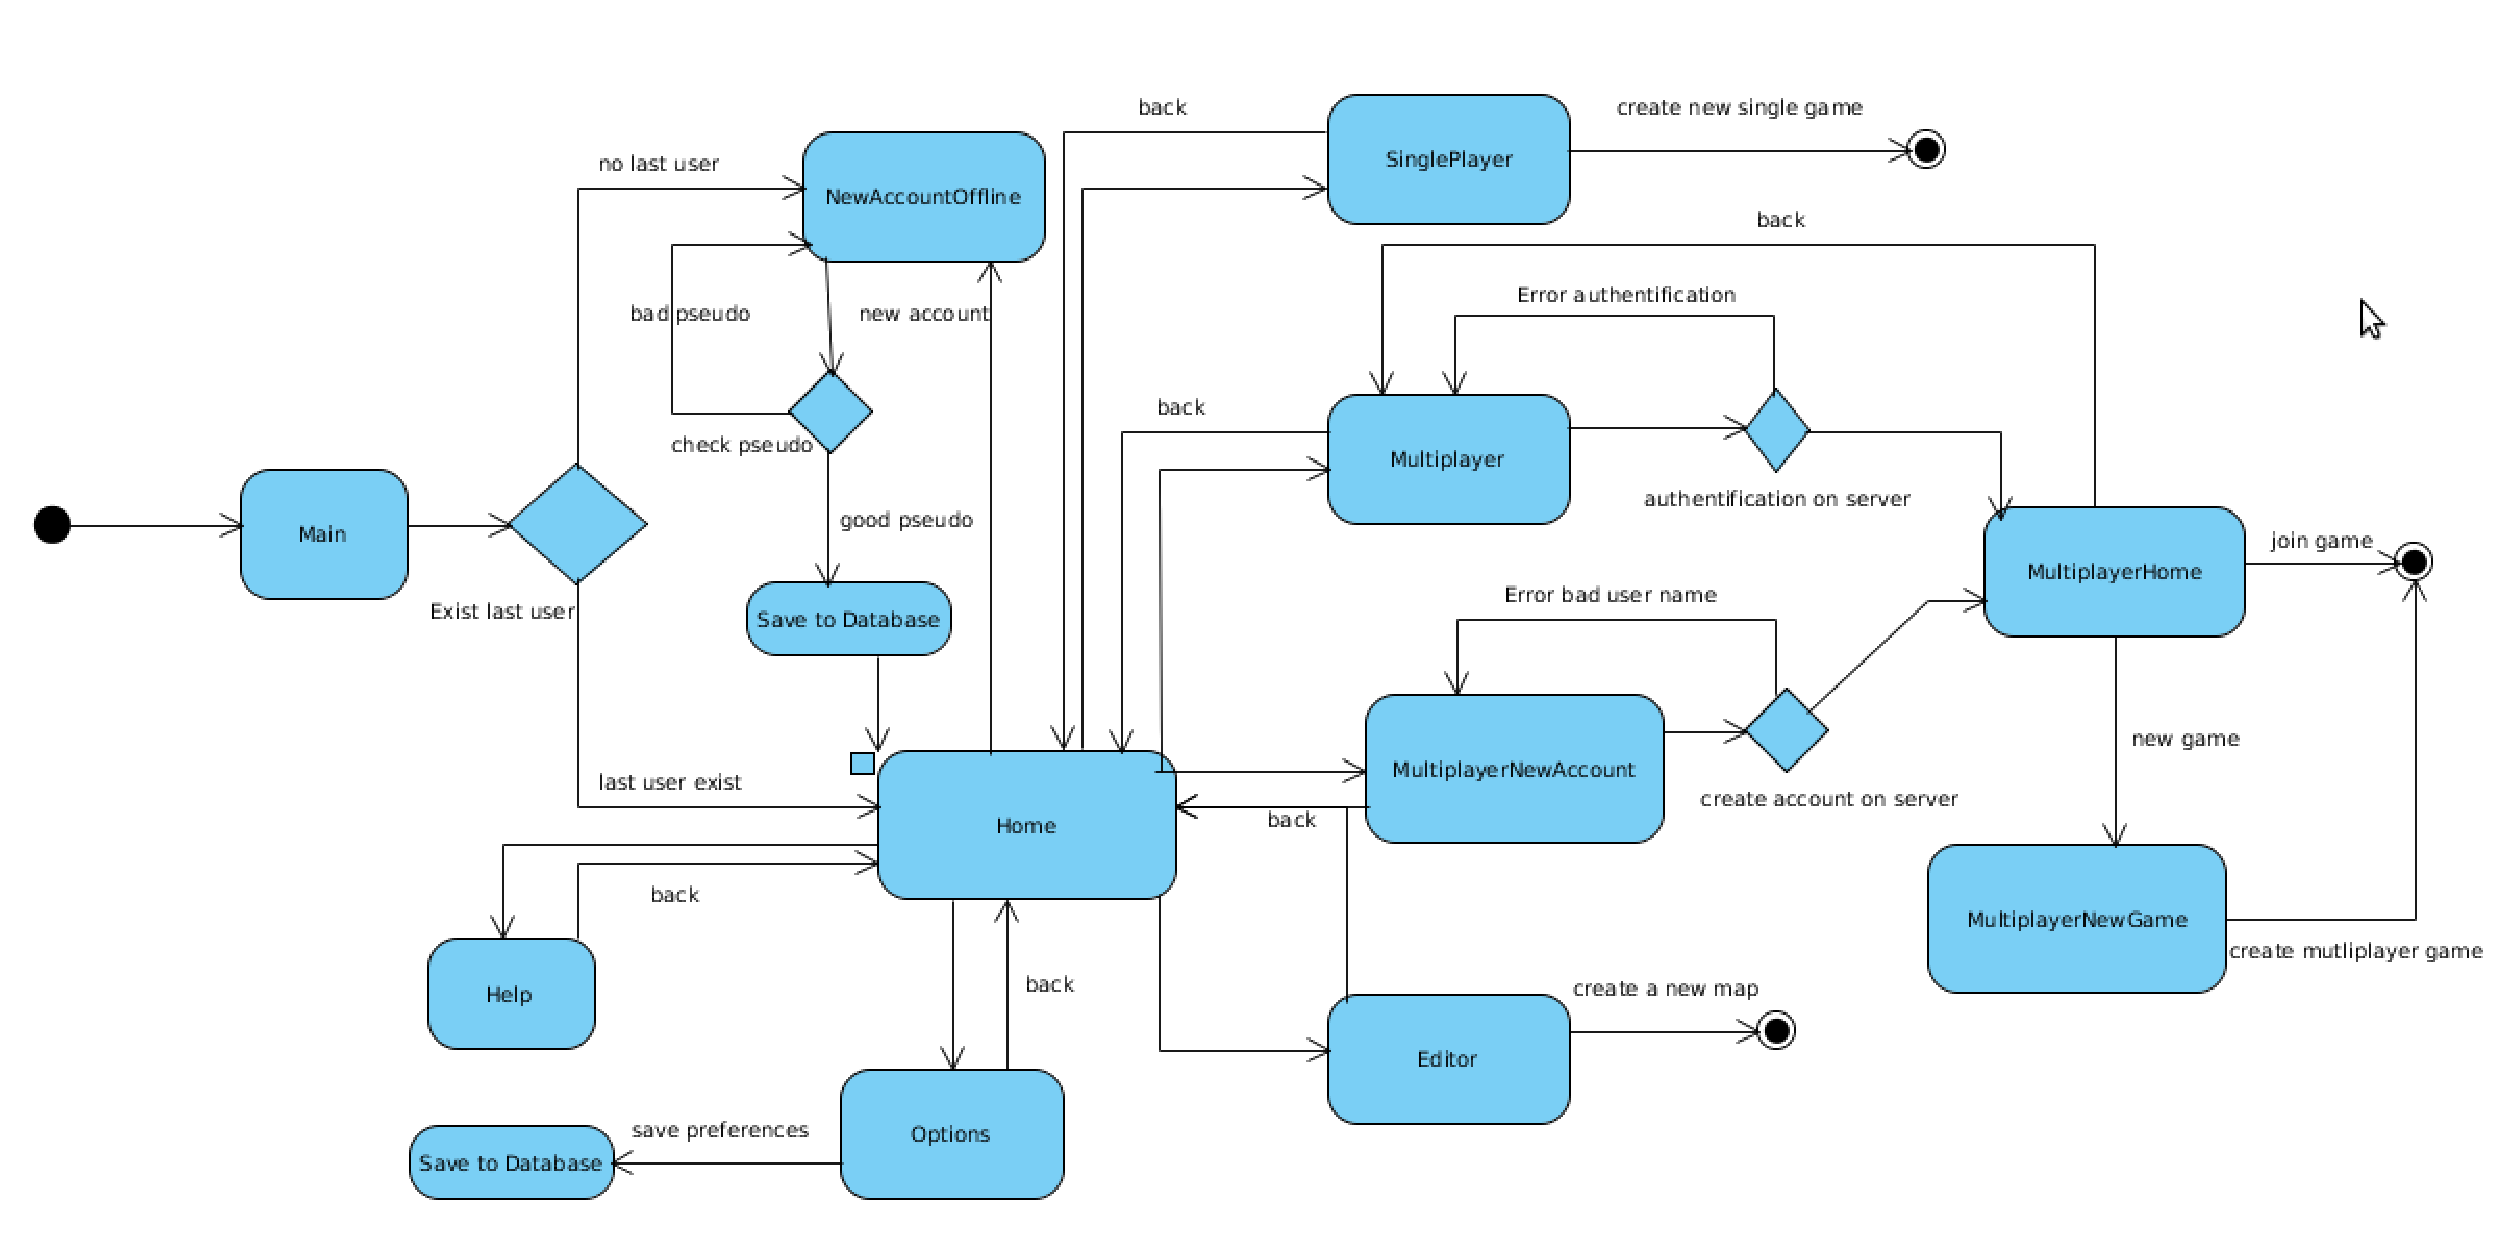
\includegraphics[width=23cm, angle=90]{Analyse/Img/diag_activity.eps}
		\caption{Diagramme d'activité}
	\end{figure}

	\paragraph{Base de données\\}
			
		Une base de données locale a elle aussi été conçue. Cette dernière a pour
		but de stocker plusieurs types de données.
				
		En effet dès lors qu'un compte local est crée sur le téléphone dans la
		table PlayerAccount, il est possible de conserver ses préférences de joueur
		tel que la couleur du joueur, le pseudonyme ou même ses paramètres de connexion multijoueur. 
		Vous pourrez créer autant de comptes locaux que vous le désirez, et il
		sera possible possible d'éditer ou choisir son compte.
				
		L'application est par ailleur en mesure de conserver
		les valeurs sonores, la langue et même le dernier utilisateur de
		l'application, grâce à un son id qui est clé étrangère dans la table System(lastUser).
				
		De plus l'application sera délivrée avec quelques cartes officielles, mais
		l'utilisateur aura libre droit de créer ses propres cartes de jeu via un
		éditeur. Elles seront alors stockées dans la table Map avec toujours une
		clé étrangère vers l'id de son créateur(owner). \\
		
		\newpage
				
		\begin{figure}
			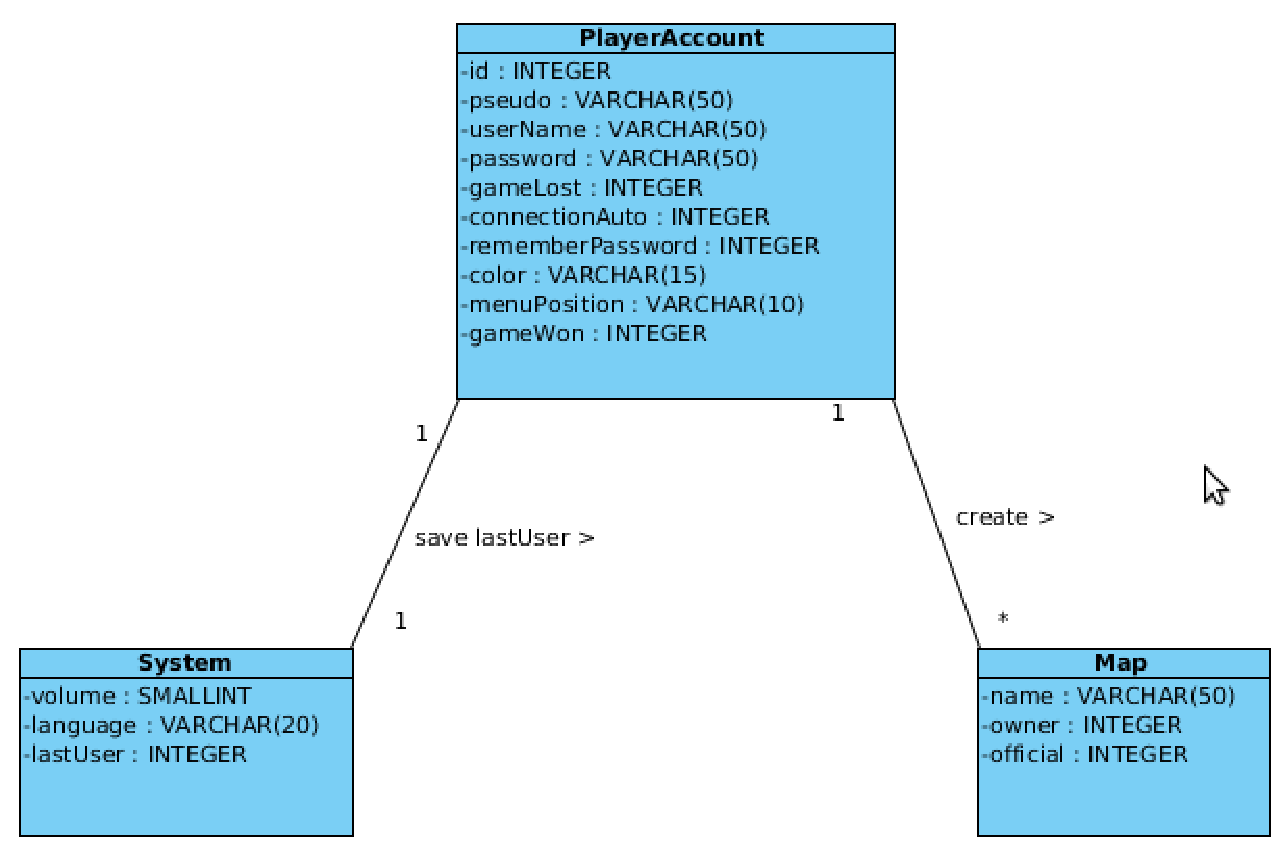
\includegraphics[width=11cm]{./Analyse/Img/menu_bdd.eps}
			\caption{Diagramme de classe Base de données}
		\end{figure}
		
		
		
						
	\paragraph{Scénarios}
	
	
\subsection{Editeur de carte}	

	L'éditeur de carte est une fonctionnalité qui va permettre à un utilisateur de créer facilement ses propres cartes pour ensuite y jouer dessus contre l'intéligence artificielle. Après avoir réfléchi sur toutes les fonctionnalités que l'éditeur de carte devait remplir, nous avons retenu celles-ci : permettre à l'utilisateur de créer une nouvelle carte, mais aussi de charger une ancienne carte précèdemment créée. Ensuite lui donner la possibilité de modifier le sol de la carte et aussi ajouter ou supprimer des blocs de la carte et enfin la dernière fonctionnalité que l'éditeur de carte implémente c'est de pouvoir placer les différents points de départ des joueurs sur la carte.
		
	Pour réaliser cette partie de l'application, nous avons utilisé le modèle de conception MVC pour diviser le code de l'éditeur de carte. Grâce a cette décomposition, le code est plus lisible et plus facile à réutiliser. 
			
	\subsubsection*{Modèle}
		La partie modèle va contenir toute les données de l'éditeur de carte. Les cartes sont les principales données qu'il va devoir manipuler. Pour cela nous avons décidé de la réprésenter sous la forme de deux matrices, la première représentant les objets du premier niveau (le sol) et la deusième la matrice du second niveau (les blocs, les points de départ des joueurs, etc).
			
			
	\subsubsection*{Vue}
		Ensuite, la vue représentera l'interface graphique de notre éditeur de carte. La principale difficulté pour réaliser l'interface graphique était de devoir rentrer toutes les informations nécessaires pour l'éditeur de carte dans un écran de type smartphone \footnote{Traduit littéralement comme \og téléphone intéligent \fg \, en français, c'est un terme utilisé pour désigner les téléphones évolués, qui possèdent des fonctions similaires à celles des assistants personnels. Certains peuvent lire des vidéos, des MP3 et se voir ajouter des programmes spécifiques.}. Après plusieurs prototypes d'interface, nous avons décide de séparer l'interface en trois parties. Tout d'abord la plus grande partie, l'affichage de la carte, qui comment étant la principale information à afficher, nous avons essayé de maximiser sa taille. Ensuite un menu à droite permettant au joueur de changer d'outil. Et la dernière partie affiche les différents éléments permettant de controler l'éditeur de carte. L'utilisateur aura juste à choisir l'outil qu'il veut placer sur la carte grâce au menu de droite et ensuite lui suffira d'appuier sur la carte pour placer un bloc dessus.
		
%		\begin{figure}
			\begin{center}
				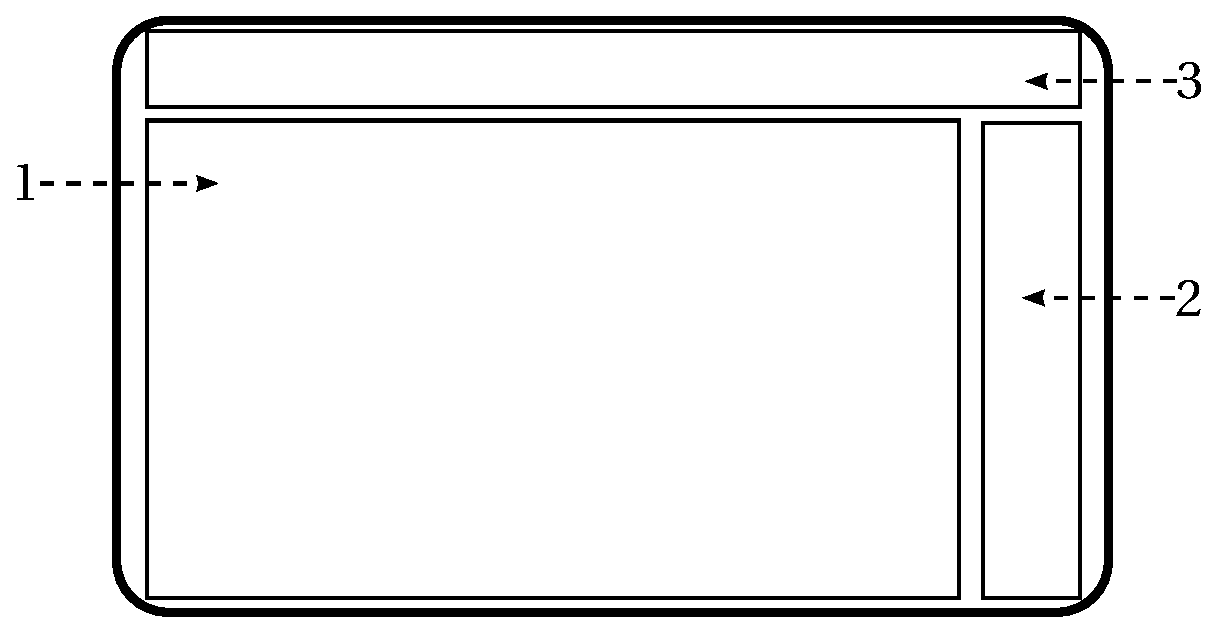
\includegraphics[width=11cm]{./Analyse/Img/14-Editeur_de_niveau.eps}
			\end{center} 
%		 	\caption{Poulpy est multicolore}
%		 	\label{Poulpy est multicolore}
%		\end{figure}
			
			
	\subsubsection*{Controleur}
		Pour finir le controleur aurra pour but de faire la liaison entre les données du modèle et de la vue. Chaque vue possède son controleur, et il y a un controleur gobal possédant les controleurs de chaque vue.
			

\subsection{Jeu}
	\subsubsection{Intelligence artificielle}
		La principale action que l'intélligence artificielle doit savoir effectuer, c'est de pouvoir se déplacer dans son environement. C'est pour cela que nous avons regardé comment déplacer un object dans un graphe, et nous avons trouvé plusieurs algorithmes, mais nous on avons retenu deux en particulé.
	
		Tout d'abord l'algorithme de recherche A* a pour but de rechercher un chemin dans un graphe entre un nœud initial et un nœud final tous deux préalablement définis. A* permet de trouver l'un des meilleurs (mais pas forcément le meilleur) chemins existant entre un point A et un point B (il retourne le premier chemin trouvé). La force de cette algorithme est le temps de calcul et l'exactitude des résultats, contrairement à Dijkstra qui est le deusième algorithme que nous avons retenu qui lui fournit toujours le meilleur résultat (le plus court chemin entre deux points) mais dans un temps d'exécution beaucoup plus long que l'algorithme de A*. Et comme il peut y avoir jusqu'à trois bots \footnote{Bot (diminutif de robot) désigne un personnage contrôlé par l'ordinateur.} et que l'intéligence artificielle doit réguliairement recalculer son chemin en fonction des actions effectuées par les autres joueurs, nous avons donc choisi l'algorithme de A*. 
	
		Maintenant que l'on sait quel algorithme utiliser pour rechercher un chemin dans un graphe, nous allons voir en détail comment marche l'algorithme de A*.
	
		Pour comprendre comment l'algorithme, nous allons nous aider d'un dessin représentent une carte avec un point A (départ) est affiché en vert, le point B (arrivée) est en rouge, et où les cases en bleu représentent le mur.
	
		\begin{center}
			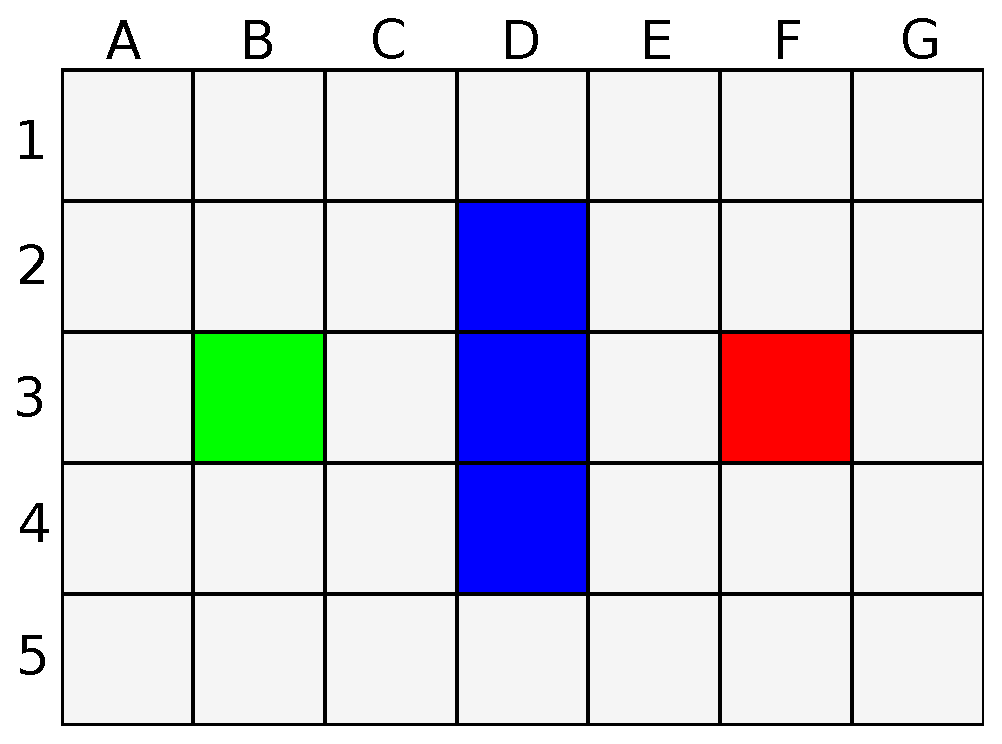
\includegraphics[width=8cm]{./Analyse/Img/Grille.eps}
		\end{center}
	
		La premier chose que l'on peut observer, c'est que la carte est divisée en cases. Chaque case de la matrice représente un node qui peut être soit traversable, soit non traversable. Dans l'application, il y que les murs ou les bombes que l'on ne peut pas traverser sinon tous les autres objets les joueurs peuvent les traverser. Donc le but de l'algorithme est de trouver un chemin entre A et B en évitant les murs. 
	
		Durant le déroulement de l'algorithme, nous avons utilisé deux listes qui contiennent des cases de la carte. Il y a une liste dite \og listeOuverte \fg \, et l'autre \og listeFermée \fg. La listeOuvrete contient une liste de cases qui pourraient éventuellement faire partie du chemin, mais pas forcément, pour le moment elle sera vide. Plus précisément c'est une liste de cases que nous devons vérifier. Ensuite, au niveau de la listeFermée, elle contient toutes les cases que nous aurons déjà vérifiées, au début de l'excution, elle contient que le point de départ (B3).
	
		Commencons les explication du déroulement de l'algorithme. Tout d'abord, il faut savoir qu'un joueur peut se déplacer dans toutes les directs, donc nous allons ajouter toutes les cases adjacentes à la listeOuvert qui sont traversable, il y en a huite (A2, B2, C2, A3, C3, A4, B4, C4). Donc pour le moment nous devons avoir ça :
	
		\begin{center}
			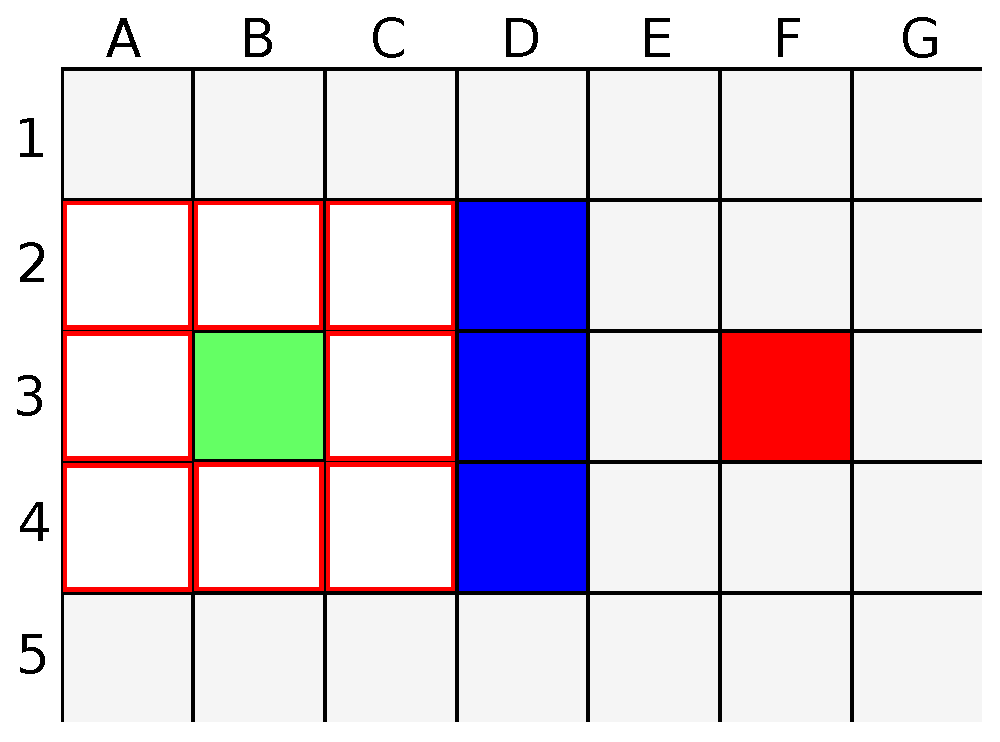
\includegraphics[width=8cm]{./Analyse/Img/Grille2.eps}
		\end{center}
	
		Les carrés avec un contour rouge sont les carrés qui sont dans la listeOuverte et les carrés qui on une couleur un peut plus foncé que les autre sont les carrés qui se trouvent dans la listeFermée.
	
		Maintenant pour choisir la case par laquelle on doit passer, nous devons rajouter trois données \og F \fg , \og G \fg \, et \og H \fg:
		\begin{description}
			\item[G : ]{c'est le coût de mouvement pour aller de la case A à une case donnée sur la grille, en suivant le chemin généré jusqu'à cette dernière.}
			\item[H :]{c'est l'heuristique, c'est à dire le coût estimé pour allé du point courant à l'arrivé. Comme nous ne connaissons pas vraiment la distance qu'il nous reste à parcourir, car toutes sortes d'obstacle peuvent se trouver sur notre chemin (objet non traversable). Donc nous allons devoir l'approximer grâce à une fonction, pour la calculer nous avons choisi d'utiliser l'heuristique de Manhattan, qui consiste à compter le nombre de bloc (à vol d'oiseau et sans prendre les diagonales) qui lui reste à parcourir.}
			\item[F :]{c'est G + H}
		\end{description} 
	
		Chaque case de la listeOuverte ou de la listeFermée vont devoir possèder toutes ces données, plus les coordonnées de leur père, c'est à dire les coordonnées de la case qui vient de les ajouter dans la la listeOuverte. Pour calculer G, nous allons assigner un coût de 10 pour chaque déplacement horizontal ou vertical, et un coût de 14 pour un mouvement en diagonale. Nous utilisons ces données car la distance nécessaire pour se déplacer est la racine carrée de 2, ou approximativement 1.41 fois le coût d'un déplacement vertical ou horizontal. Nous utiliserons donc 10 et 14 pour des raisons de simplification. Par conséquent, nous allons multiplier par 10 le coût H pour qu'il soit cohérent par rapport à G.

		Donc maintenant, nous devons avoir cette matrice :
		\begin{center}
			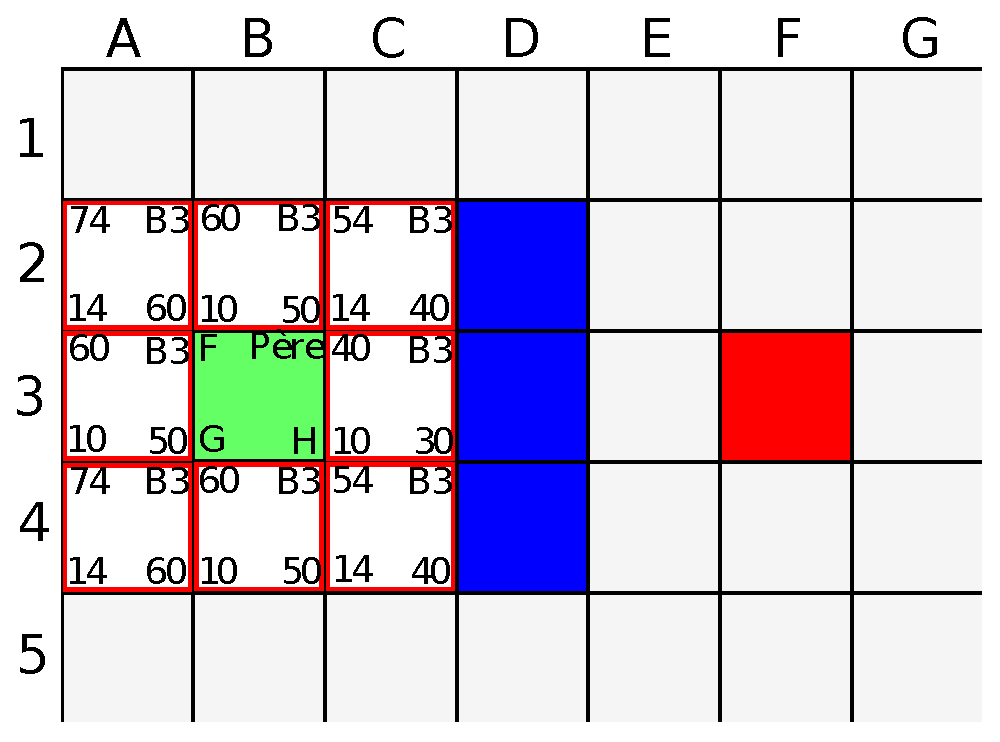
\includegraphics[width=8cm]{./Analyse/Img/Grille3.eps}
		\end{center}
	
		Après avoir ajouté toutes les cases adjacentes à la case courant, il suffit de prendre la case qui a le plus petit coût F et ensuite de la rajouter dans la listeFermée et de la supprimer de la listeOuverte. Nous obtenons donc :
		\begin{center}
			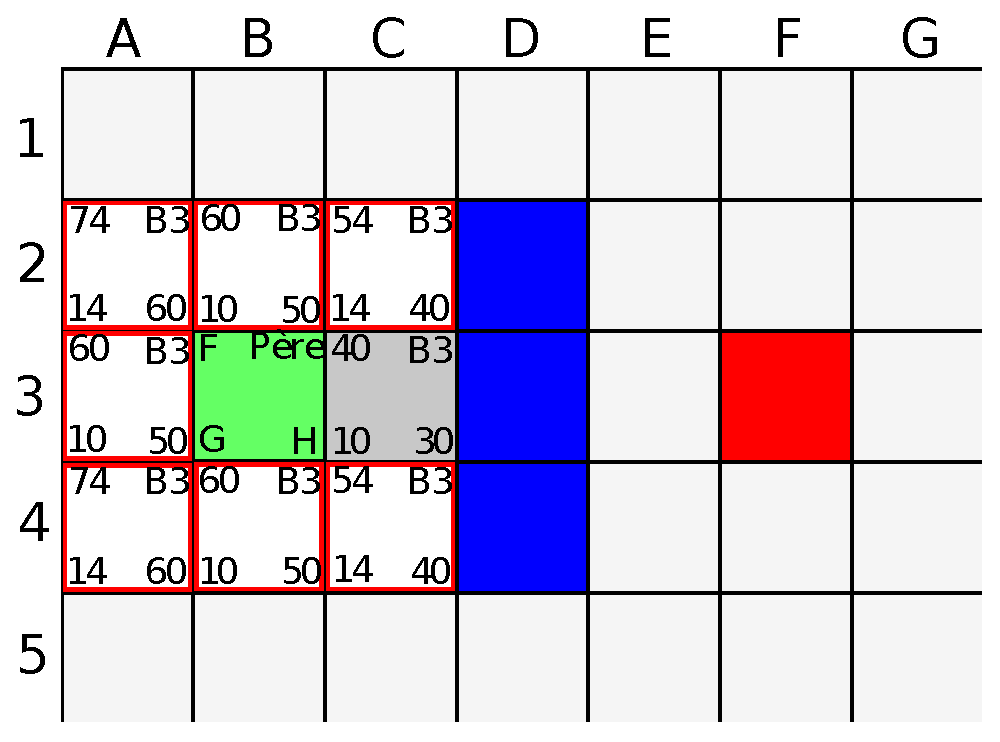
\includegraphics[width=8cm]{./Analyse/Img/Grille4.eps}
		\end{center}
	
		Ensuite on regarde toutes les cases adjacentes à la dernière case ajoutée dans la listeFermée. Si elles se trouvent déjà dans la listeOuverte, on vérifit que leurs coût soient inférieur au coût de la case correspondante déjà dans la listeOuverte, si oui alors on la remplace sinon on ne fait rien.
	
		Pour finir on répète cette opération jusqu'on arrive à la case d'arrivée, nous obtenons ça :
		\begin{center}
			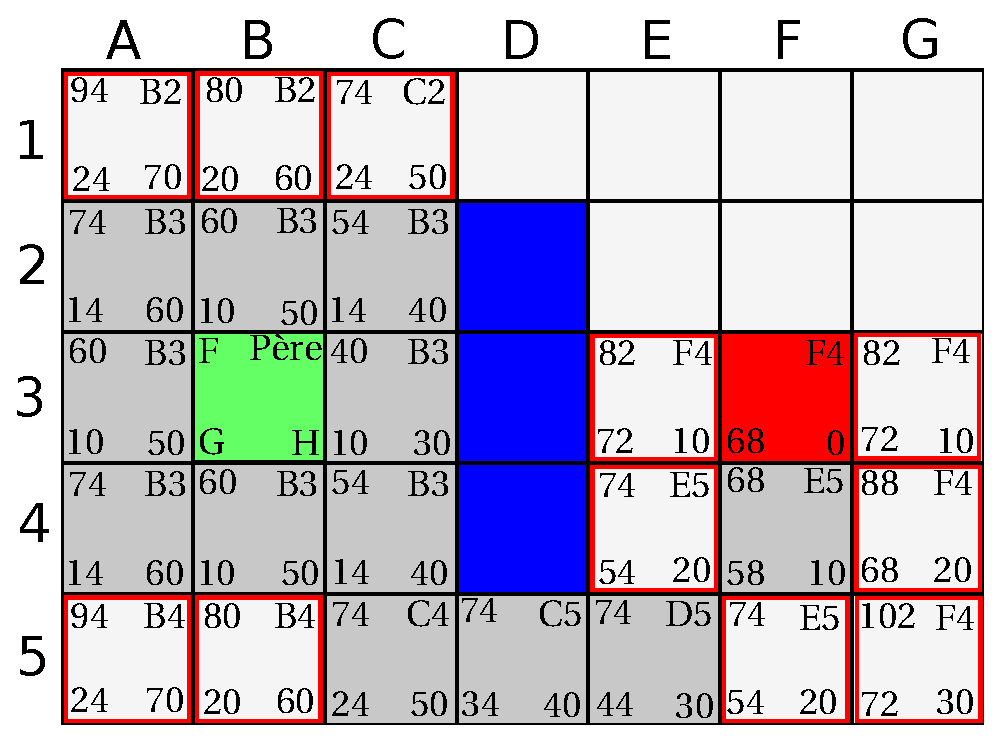
\includegraphics[width=8cm]{./Analyse/Img/Grille5.eps}
		\end{center}
	
		Pour finir, il nous suffit juste de récupérer la case d'arrivée et de regarder son père, puis de repéter cette opération avec la case obtenu jusqu'à arriver à la case de dépard. Grâce à ça nous obtenons cette dernière étape de l'algorithme :
		\begin{center}
			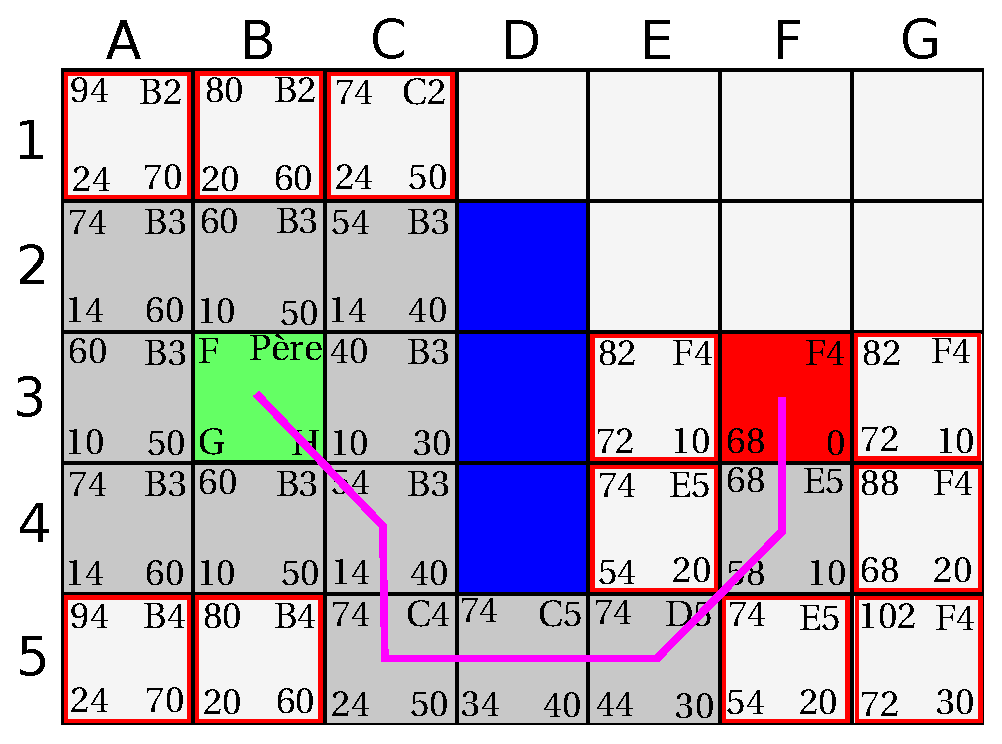
\includegraphics[width=8cm]{./Analyse/Img/Grille6.eps}
		\end{center}
	
		Comme on peut le voir sur le schéma prèdédent, le chemin qu'à trouvé l'algorithme de A* est le suivant : $ B3 \rightarrow C4 \rightarrow C5 \rightarrow D5 \rightarrow E5 \rightarrow F4 \rightarrow F3 $. L'algorithme aurait pu d'autre chemin équivalent à celui-ci mais le principe de cette algorithme c'est de renvoyer le permier chemin qu'il trouve.
			

\subsection{Réseau}
		
	\paragraph{Serveur\\}
			
		Il a été fixé dans le cahier des charges que notre serveur devrait pouvoir
		effectuer plusieurs tâches particulières séparées. Nous avons donc décidé de
		les compartimenter en classes.
		
		Notre serveur est crée sur une base de servlet. Ce fût ici
		aussi un point nouveau pour nous, réiterant les phases d'analyse, de
		découverte, de test et de mise en place. Le fonctionnement est basé sur les
		échanges de requêtes type HTTP, où à chaque demande correspond une réponse. 
		
		Une servlet est une classe Java qui permet de créer dynamiquement des données
		au sein d'un serveur HTTP. Une servlet s'exécute dynamiquement sur le serveur
		web et permet l'extension des fonctions de ce dernier, typiquement : accès à
		des bases de données.
			
		Les six éléments situés sur la partie haute du schéma
		ci-dessous(respectivement ServletInscription, ServletConnection,
		ServletGamesList, ServletCreateGame, ServletConnectionGame et
		ServletManageGame), représente les différentes tâches qu'un utilisateur
		puisse demander au serveur. Elles sont reliées à une classe nommée
		ContextListener, qui leur permettra d'accéder aux mêmes données sans qu'il y
		ait de conflits. La partie basse représente les objets qui seront utilisés pour les parties en multijoueurs. 
		Bien évidemment ces objets sont très proches de ceux utilisés dans les parties
		locales(Schéma 3.3).
		
		
		Comme il a été dit précédement, notre serveur est accessible via des requêtes
		HTTP contactant des servlets. Ces servlets sont stockées dans un serveur
		d'application nommé Apache Tomcat. Il s'agit d'un conteneur libre de
		servlets Java 2 Enterprise Edition, mais il fait aussi office de serveur
		Web.\\
		
		
		Le scénarios le plus probable serait le suivant. Un utilisateur désire jouer
		en ligne contre de vrais joueurs. 
		Il va alors passer par l'inscription et créer son compte sur le
		serveur(Inscription). Une fois cette étape obligatoire faite, il pourra
		choisir entre rejoindre une partie en ligne en cour(ConnectionGame), ou en
		créer un nouvelle(CreateGame). Dès lors qu'il aura accès à une partie en
		ligne, un contact régulier avec le serveur sera obligatoire afin de réaliser
		les interactions entre les différents joueurs(ManageGame). Tout ceci devra se
		réaliser bien sûr dans une durée infime afin de ne pas pénaliser les joueurs.	
		
		\begin{figure}
			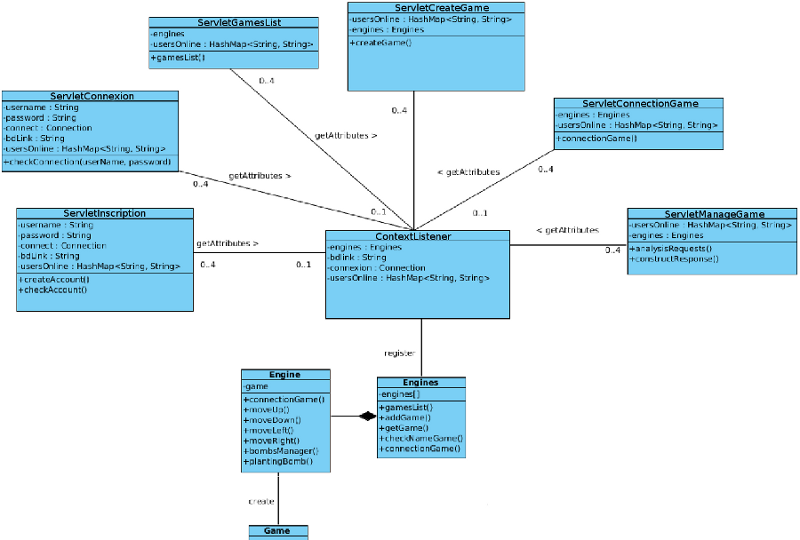
\includegraphics[scale = 0.5]{Analyse/Img/serveur.eps}
			 \caption {Serveur}
		\end{figure}
		
		\newpage
		
		
	\paragraph{JSON\\}	
		Soucieux des performances et de la rapidité des échanges entre applications et
		serveur, nous avons mis en place un protocole de communication client/serveur
		où les messages transitant sont des flux JSON\footnote{JavaScript Object
		Notation :  format de données textuel issu du JavaScript (ECMAScript pour plus
		exact) où il était employé comme une syntaxe pour décrire les valeurs des
		instances d’objets}. 	
		Contrairement au XML qui peut représenter des données orientées document,
		JSON se focalise sur la description d’objets.
		Un autre avantage reconnu de JSON par rapport à XML est qu’il est nettement
		moins verbeux que ce dernier.
		Quoi qu’il en soit JSON reconnait la philosophie des services web exposant
		une interface d’échange : il s’agit
		d’envoyer et de recevoir des informations dans un format facilement manipulable par
		le protocole de transport HTTP.
		
		
		Voilà pourquoi le JSON semblait être un format de données d'échanges optimal
		pour véhiculer le plus d'informations avec une taille moindre. Il est aussi en
		adéquation avec notre politique d'utilisation web pour un serveur.
		De plus étant beaucoup utilisé, nos deux
		langages mettent à disposition des outils de sérialisation de leurs objets en JSON.
		
		Ci-dessous un exemple concret de notre protocole de communication JSON entre
		serveur et application cliente.
		
			
		\begin{verbatim}
			ServletInscription
				Player => Serveur
				{["username","password"]}
				
				Serveur => Player
				{"OK"} ou {"BU"}
				
			ServletConnexion 	
				Player => Serveur
				{["username","password"]}
				
				Serveur => Player
				{"OK"} ou {"BU"}
				
			ServletGameList
				Player => Serveur
				{"userKey"}
			
				Serveur => Player
				{[{"class":"Game","map":"mapName","name":"gameName",
				 "playerNumberConnected":nbConnected,"type":"gameType"},{..},{..}]}
				 
			ServletCreateGame:
				Player => Server:
					{"userKey": <userKey>, 
					"game": {"name":<name>, "type":<type>, "map":<map>, "ennemiesNumber": <ennemiesNumber>}}
					
				Server => Player:
					{"OK"} ou {"errorType"}
				 
			ServletConnectionGame:
				Player => Server:
					{["userKey", "gameName"]}
					
				Server => Player:
					{[<1/2/3/4>, "play<true/false>", "map", "time<mm:ss>"]} 
					ou 
					{"errorType"}
					
			ServletManageGame:
				Player => Server: 
					{"userKey", "gameName", "action"}	
					
				Server => Players: (Player, bombs, blocs, score, time)
					{[
					 [ ["x", "y", "direction", "dead <true/false>"],[...] ],
					 [ ["x", "y", "type", "explode <true/false>" ], [...] ],
					 [ ["position": {"x", "y"}, "bonus": <bonus>], [..] ],
					 [1,2,3,4],
					 "time <mm:ss>"]} 
					 ou 
					{"errorType"}
				 
				 
		\end{verbatim}
			
		
	

	\subsubsection{Schéma de fonctionnement }
		
		\begin{center}
			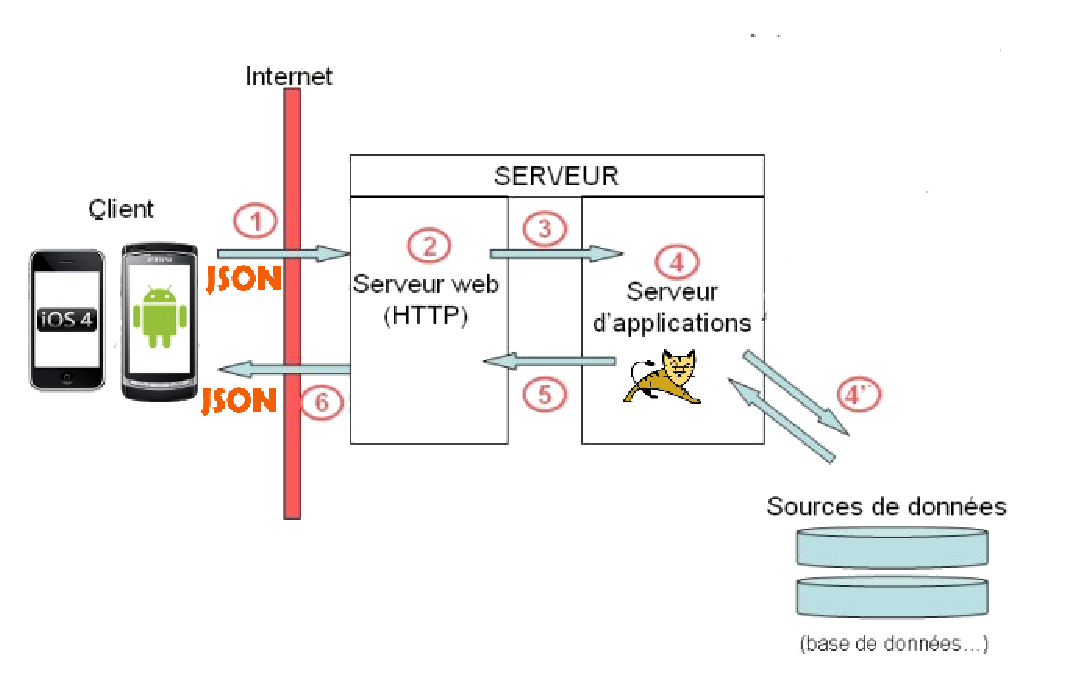
\includegraphics[width=16cm]{Analyse/Img/serveurappli.eps}
		\end{center}
		
		\begin{enumerate}

			\item 
					Le client émet une requête pour demander une
					ressource au serveur. Par exemple la création de son compte multijoueur,
					qui pourrait se situer \url{http://Bomberklob.com/inscription}
			\item
					Côté serveur, c'est le serveur web qui traite les
					requêtes HTTP entrantes. Il traite donc toutes les requêtes, qu'elles
					demandent une ressource statique ou dynamique. Seulement, un serveur HTTP
					ne sait répondre qu'aux requêtes visant des ressources statiques.

			\item 
					Ainsi, si le serveur HTTP s'aperçoit que la requête reçue est destinée
					au serveur d'applications, il la lui transmet. Les deux serveurs sont
					reliés par un canal, nommé connecteur.
		
			\item
					Le serveur d'applications (dans notre cas Tomcat) reçoit la requête à
					son tour. Lui est en mesure de la traiter. Il exécute donc la servlet
					correspondante à la requête, en fonction de l'URL, en récupérant les
					valeurs dans le flux JSON entrant. Cette opération est effectuée à partir
					de la configuration du serveur, grâce un fichier web.xml faisant le mapping
					entre URL et servlet associée.
		
					La servlet est donc invoquée, et le serveur lui fournit notamment deux
					objets Java exploitables: un représentant la requête, l'autre représentant
					la réponse. La servlet execute sa fonction et génère la réponse à la
					demande, sous forme de flux JSON. Cela peut passer par la consultation de
					sources de données, comme des bases de données (4' sur le schéma).		
		
		\end{enumerate}
		
	\paragraph{Base de données\\}
		Afin de pouvoir conserver les utilisateurs en ligne ainsi que leurs infos
		personnels et permettre une authentification, nous avons dû établir une
		base de données sur le serveur. Cette dernière à été pensé comme demandé pour 
		l'enregistrement de comptes. Une unique table nommée Users remplie donc cette
		fonction. Le serveur devra pouvoir y accéder en écriture(inscription) comme
		en lecture(connexion).
			
		Elle ne comportera que deux champs, userName et password. Dès lors que
		l'utilisateur désirera créer un compte multijoueur, il renseignera dans
		l'application son userName souhaité ainsi que son mot de passe. 
		Ce couple sera 	alors envoyé au serveur qui vérifiera dans cette base de
		données, que le userName(unique) n'est pas déjà utilisé. Auquel cas un nouveau n-uplet sera
		inséré et permettra l'authentification de l'utilisateur par la suite. Les mots
		de passe seront bien évidement crypté pour des raisons de sécurité.
			
		
		
		\newpage
		
	